\documentclass[xcolor=pdftex,dvipsnames,table,mathserif]{beamer}
%\usepackage{subfigure}
\usepackage{amsbsy}
\usepackage{tikz}
\usetikzlibrary{arrows}
\usepackage{amsmath,graphicx,dsfont,color}
\usepackage{amsfonts}
\usepackage{amssymb}
\usepackage{array}

\usepackage{subfig}

% makes the subfig package work
\makeatletter
\let\@@magyar@captionfix\relax
\makeatother

% subfigure counter resets every frame
\makeatletter
\@addtoreset{subfigure}{framenumber}
\makeatother

% First author and year
\bibliographystyle{apalike}

% This sets the list items of the bibliography to the same symbol used for citation.
\setbeamertemplate{bibliography item}{\insertbiblabel}

% This avoids extralines for different entries
\setbeamertemplate{bibliography entry title}{}
\setbeamertemplate{bibliography entry location}{}
\setbeamertemplate{bibliography entry note}{}

\DeclareMathOperator*{\argmin}{arg\,min}
\DeclareMathOperator*{\argmax}{arg\,max}
%Definitiona

\newcommand{\x}{\mathbf{x}}
\newcommand{\X}{\mathbf{X}}
\newcommand{\W}{\mathbf{W}} %Weight
\newcommand{\bais}{\mathbf{b}}%Bais
\newcommand{\act}{\texttt{g}}%Activation
\newcommand{\loss}{L}
\newcommand{\pdata}{\hat{p}_{\texttt{data}}}
\newcommand{\nsize}{N}
\newcommand{\nfeatures}{P}
\newcommand{\param}{\boldsymbol{\theta}}
\newcommand{\featmap}{\boldsymbol{\phi}}
\newcommand{\EV}{\mathbb{E}}







\usepackage{physics}
\usepackage{tikz}
\usepackage{algorithm,algorithmic}
\usetikzlibrary{fit,positioning}

%% \usepackage{animate}

\AtBeginSection[]{
  \begin{frame}{Contents}
  \tableofcontents[currentsection, hideothersubsections]
  \end{frame}
}

\AtBeginSubsection[]{
  \begin{frame}{Contents}
  \tableofcontents[currentsection, subsectionstyle=show/shaded/hide]
  \end{frame}
}

\setbeamertemplate{footline}[frame number]{}
\setbeamertemplate{navigation symbols}{}
\setbeamertemplate{section in toc}[square]
\setbeamertemplate{items}[square]

\title{Optimization on Deep Learning}
\author{Santiago VELASCO-FORERO \\ \href{http://cmm.ensmp.fr/~velasco/}{http://cmm.ensmp.fr/~velasco/}}
\date{MINES ParisTech\\
  PSL Research University\\
  Center for Mathematical Morphology
}
\titlegraphic{
\includegraphics[height=1.7cm]{../graphics/logoemp}}

\useinnertheme{rounded}
\usecolortheme{rose}

%%%%%%%%%%%%%%%%%%%%%%%%%%%%%%%%%%%%%%%%%%%%%%%%%%
%%%%%%%%%%%%%%%%%%%%%%%%%%%%%%%%%%%%%%%%%%%%%%%%%%
\begin{document}
\begin{frame}
\titlepage
\end{frame}

\frame{
\frametitle{Contents}
\tableofcontents[]
}


%%%%%%%%%%%%%%%%%%%%%%%%%%%%%%%%%%%%%%%%%%%%%%%%%%
\section{Introduction}


\section{Stochastic Gradient Descent}

%\begin{frame}{Stochastic Gradient Descent (SGD) update \cite{robbins1985stochastic}}
%\begin{itemize}
%\item \textbf{Require}: Learning rate $\epsilon$ (or a learning rate schedule)
%\item \textbf{Initialization}: $k=1$, $\param_1$ some random value.
%\item \textbf{while} stopping criterion not met \textbf{do}
%\item \quad\quad\quad\textbf{Sample} a value from the training set $(x^{(0)},y^{(0)})$
%\item \quad\quad\quad\textbf{Gradient} $\mathbf{g}(\param_{t}) =\frac{\partial  L(f(x^{(0)},\param_i),y^{(0)})}{ \partial{\param}}$
%\item \quad\quad\quad\textbf{Update} $\param_{t+1}= \param_{t}-\epsilon \mathbf{g}(\param_{t})$
%\item \quad\quad\quad\textbf{} $k=k+1$
%\end{itemize}
%\end{frame}
%
%\begin{frame}{MiniBatch Stochastic Gradient Descent (MSGD) update}
%\begin{itemize}
%\item \textbf{Require}: Learning rate $\epsilon$ (or a learning rate schedule)
%\item \textbf{Initialization}: $k=1$, $\param_1$ some random value.
%\item \textbf{while} stopping criterion not met \textbf{do}
%\item \quad\quad\quad\textbf{Sample} $m$ examples from the training set $\{ (x^{(0)},y^{(0)}),(x^{(1)},y^{(1)}),\ldots,(x^{(m)},y^{(m)})\}$
%\item \quad\quad\quad\textbf{Gradient} $\mathbf{g}(\param_{t}) =\frac{1}{m}\frac{\partial  \sum_{i=0}^{m}L(f(x^{(i)},\param_i),y^{(i)})}{ \partial{\param}}$
%\item \quad\quad\quad\textbf{Update} $\param_{t+1}= \param_{t}-\epsilon \mathbf{g}(\param_{t})$
%\item \quad\quad\quad\textbf{} $k=k+1$
%\end{itemize}
%Of $m=n$ then we get the BSGD.
%\end{frame}
%
%\begin{frame}{Learning Rate}
%INCLUDE FIGURE
%\end{frame}

\section{Optimizers}

\begin{frame}{Intuition: Gradient Descent \cite{Cauchy47}}
Goal: Minimize $f(x)$ (evaluate \alert{as few times as possible} the function $f$)\\
The Taylor series of a real $f(x)$ that is infinitely differentiable at a real $x+\epsilon$ is the power series
\begin{eqnarray*}
f(x+\epsilon)=f(x)+f'(x)\epsilon+\frac{f''(x)}{2}\epsilon^2+\dots \\
\approx f(x)+f'(x)\epsilon
\end{eqnarray*},
by considering $\epsilon= -\eta f'(x)$ for small $\eta$, we have
\begin{eqnarray*}
f(x- \eta f'(x)) \approx f(x)-f'(x)\eta f'(x) =   f(x)-\eta f'(x)^ 2  \\
f(x-\eta f'(x)) < f(x)
\end{eqnarray*}
Intuitively, since the first-order approximation is good only for small $\epsilon$, we want to choose a small $\eta > 0$ to make $\epsilon$ small in magnitude.
Thus, if our goal is to minimise $f$, we can update
\begin{equation}
x_{i+1}=x_i-\eta f'(x)
\end{equation}
where $\eta \in \mathbb{R}^{+}$ is called \emph{learning rate}.
\end{frame}

\begin{frame}{Gradient Descent \cite{Cauchy47}}
\begin{algorithm}[H]
\begin{algorithmic}[1]
\STATE \textbf{given} initial learning rate $\eta \in \mathbb{R}$ and dataset $\X$
\STATE \textbf{initialize} time step $t=0$, parameter vector $\param_{t=0} \in \mathbb{R}^\nfeatures$,
\REPEAT
\STATE t=t+1
\STATE $\mathbf{g}_t = \nabla f_i(\X,\param_{t-1})$  \begin{tiny}\texttt{Return parameter gradient}\end{tiny}
\STATE $\param_t=\param_{t-1}  - \eta \mathbf{g}_t$
\UNTIL stopping criterion is met
\RETURN optimized parameters $\param_i$
\end{algorithmic}
\caption{pseudocode gradient descent }
\label{alg:seq}
\end{algorithm}
Who is $f$ in deep learning? $\mathbb{E}_{\alert{(\mathcal{X},\mathcal{Y})}} [\loss_{\param}(\x,y)]$ for a given loss function $\loss$ 
\end{frame}

\begin{frame}{SGD \cite{robbins1985stochastic}}
\begin{algorithm}[H]
\begin{algorithmic}[1]
\STATE \textbf{given} initial learning rate $\eta \in \mathbb{R}$ and dataset $\X$
\STATE \textbf{initialize} time step $t=0$, parameter vector $\param_{t=0} \in \mathbb{R}^\nfeatures$,
\REPEAT
\STATE t=t+1
\STATE $\alert{\X_t=\texttt{SelectBatch} (\X)}$ \begin{tiny}\texttt{Select a batch from data, whole data, only one, ... } \end{tiny}
\STATE $\mathbf{g}_t = \nabla f_i(\alert{\X_t},\param_{t-1})$  \begin{tiny}\texttt{Return parameter gradient}\end{tiny}
\STATE $\param_t=\param_{t-1}  - \eta \mathbf{g}_t$
\UNTIL stopping criterion is met
\RETURN optimized parameters $\param_i$
\end{algorithmic}
\caption{pseudocode for stochastic gradient descent }
\label{alg:seq}
\end{algorithm}
\end{frame}


\begin{frame}{$\texttt{SelectBatch} (\X)$}
\begin{enumerate}
\item Vanilla gradient descent, a.k.a. \emph{batch gradient descent}, computes the gradient of the cost function w.r.t. to the parameters $\param$
for the entire training dataset.
\item \emph{Stochastic gradient descent} (SGD) in contrast performs a parameter update for each training example. 
\item \emph{Mini-batch gradient descent} performs an update for every mini-batch of $\nsize$ training examples.
\end{enumerate}
\textit{Some} difficulties:
\begin{enumerate}
\item Choosing a proper learning rate can be difficult.
\item Same learning rate applies to all parameter updates
\item Highly non-convex error functions common for neural networks is avoiding getting trapped in their numerous suboptimal local minima.
\end{enumerate}
\end{frame}


\begin{frame}{Difficulties in Deep Network Optimisation}
\begin{itemize}
\item[A]{Local minima / Global minima}
\item[B]{Saddle Point (Plateaus or Flat Regions)}
\end{itemize}
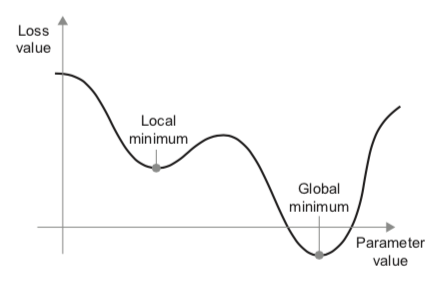
\includegraphics[width=.45\columnwidth]{../graphics/LocalGlobalMinimum}
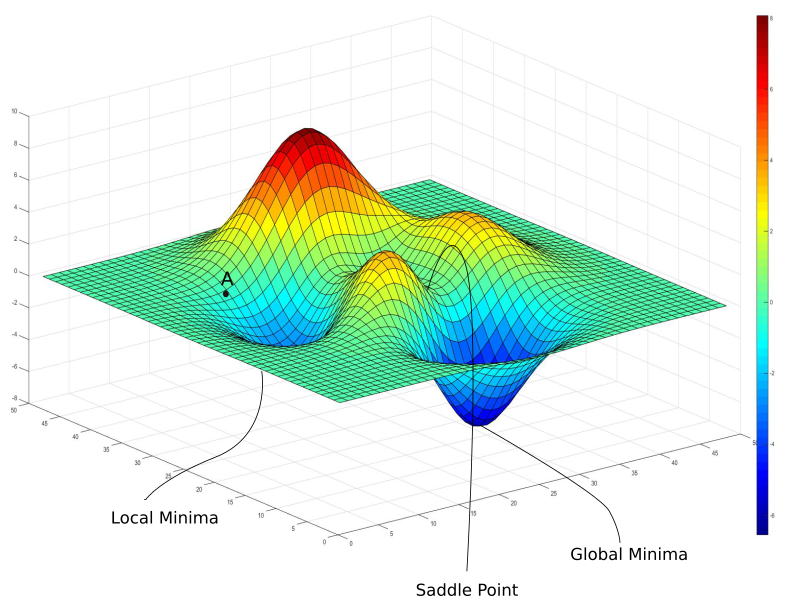
\includegraphics[width=.45\columnwidth]{../graphics/challenges1} \\

\end{frame}




\begin{frame}{Learning Rate}
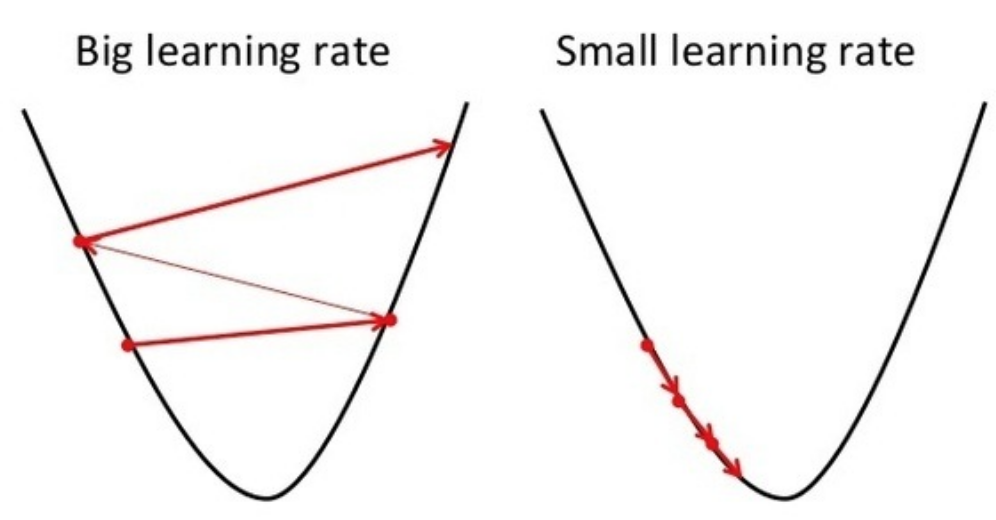
\includegraphics[width=.95\columnwidth]{../graphics/BigLearningRate}
\end{frame}

\begin{frame}{Learning Rate in Training Process}
\begin{figure}
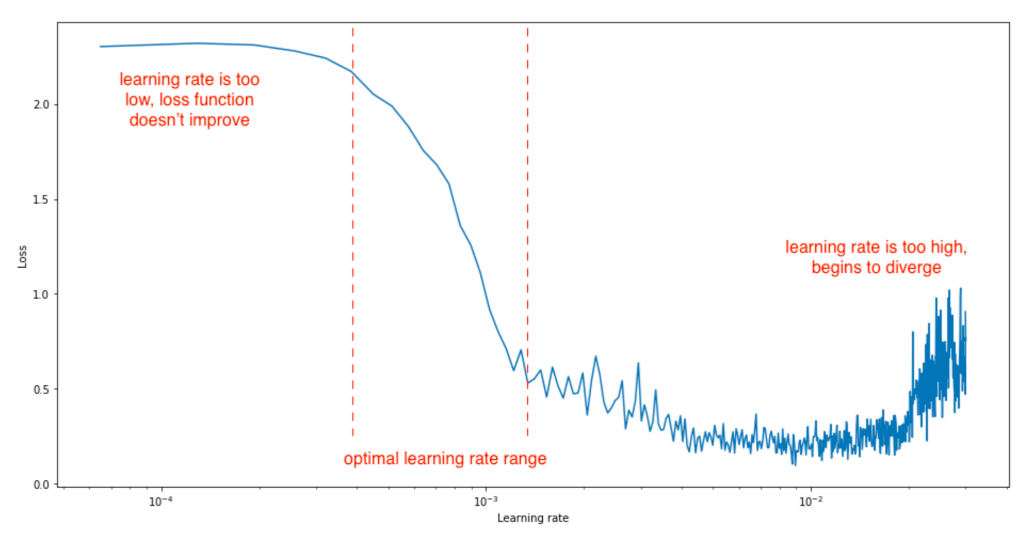
\includegraphics[width=.95\columnwidth]{../graphics/LearningRateEffect}
\end{figure}
\texttt{Image by Jeremy Jordan via https://www.jeremyjordan.me/nn-learning-rate/}
\end{frame}

\begin{frame}{SGD with Learning Rate Schedule}
\begin{algorithm}[H]
\begin{algorithmic}[1]
\STATE \textbf{given} initial learning rate $\eta \in \mathbb{R}$ and a dataset $\X$
\STATE \textbf{initialize} time step $t=0$, parameter vector $\param_{t=0} \in \mathbb{R}^\nfeatures$, schedule multiplier $\eta_{t=0} \in \mathbb{R}$
\REPEAT
\STATE t=t+1
\STATE $\X_t=\texttt{SelectBatch} (\X)$ \begin{tiny}\texttt{Select a batch from data, whole data, only one, ... } \end{tiny}
\STATE $\mathbf{g}_t = \nabla f_i(\X_t,\param_{t-1})$  \begin{tiny}\texttt{Return parameter gradient}\end{tiny}
\STATE \alert{$\eta_t = $ SetScheduleMultiplier$(t)$} \begin{tiny}{Can be fixed,decay, warm restarts, ...}\end{tiny}
\STATE $\param_t=\param_{t-1}  - \alert{\eta_{t}} \eta \mathbf{g}_t$
\UNTIL stopping criterion is met
\RETURN optimized parameters $\param_i$
\end{algorithmic}
\caption{pseudocode for SGD with Learning Rate Schedule}
\label{alg:seq}
\end{algorithm}
\end{frame}

\begin{frame}{Visualizing the Loss Landscape of Neural Net}
\begin{figure}
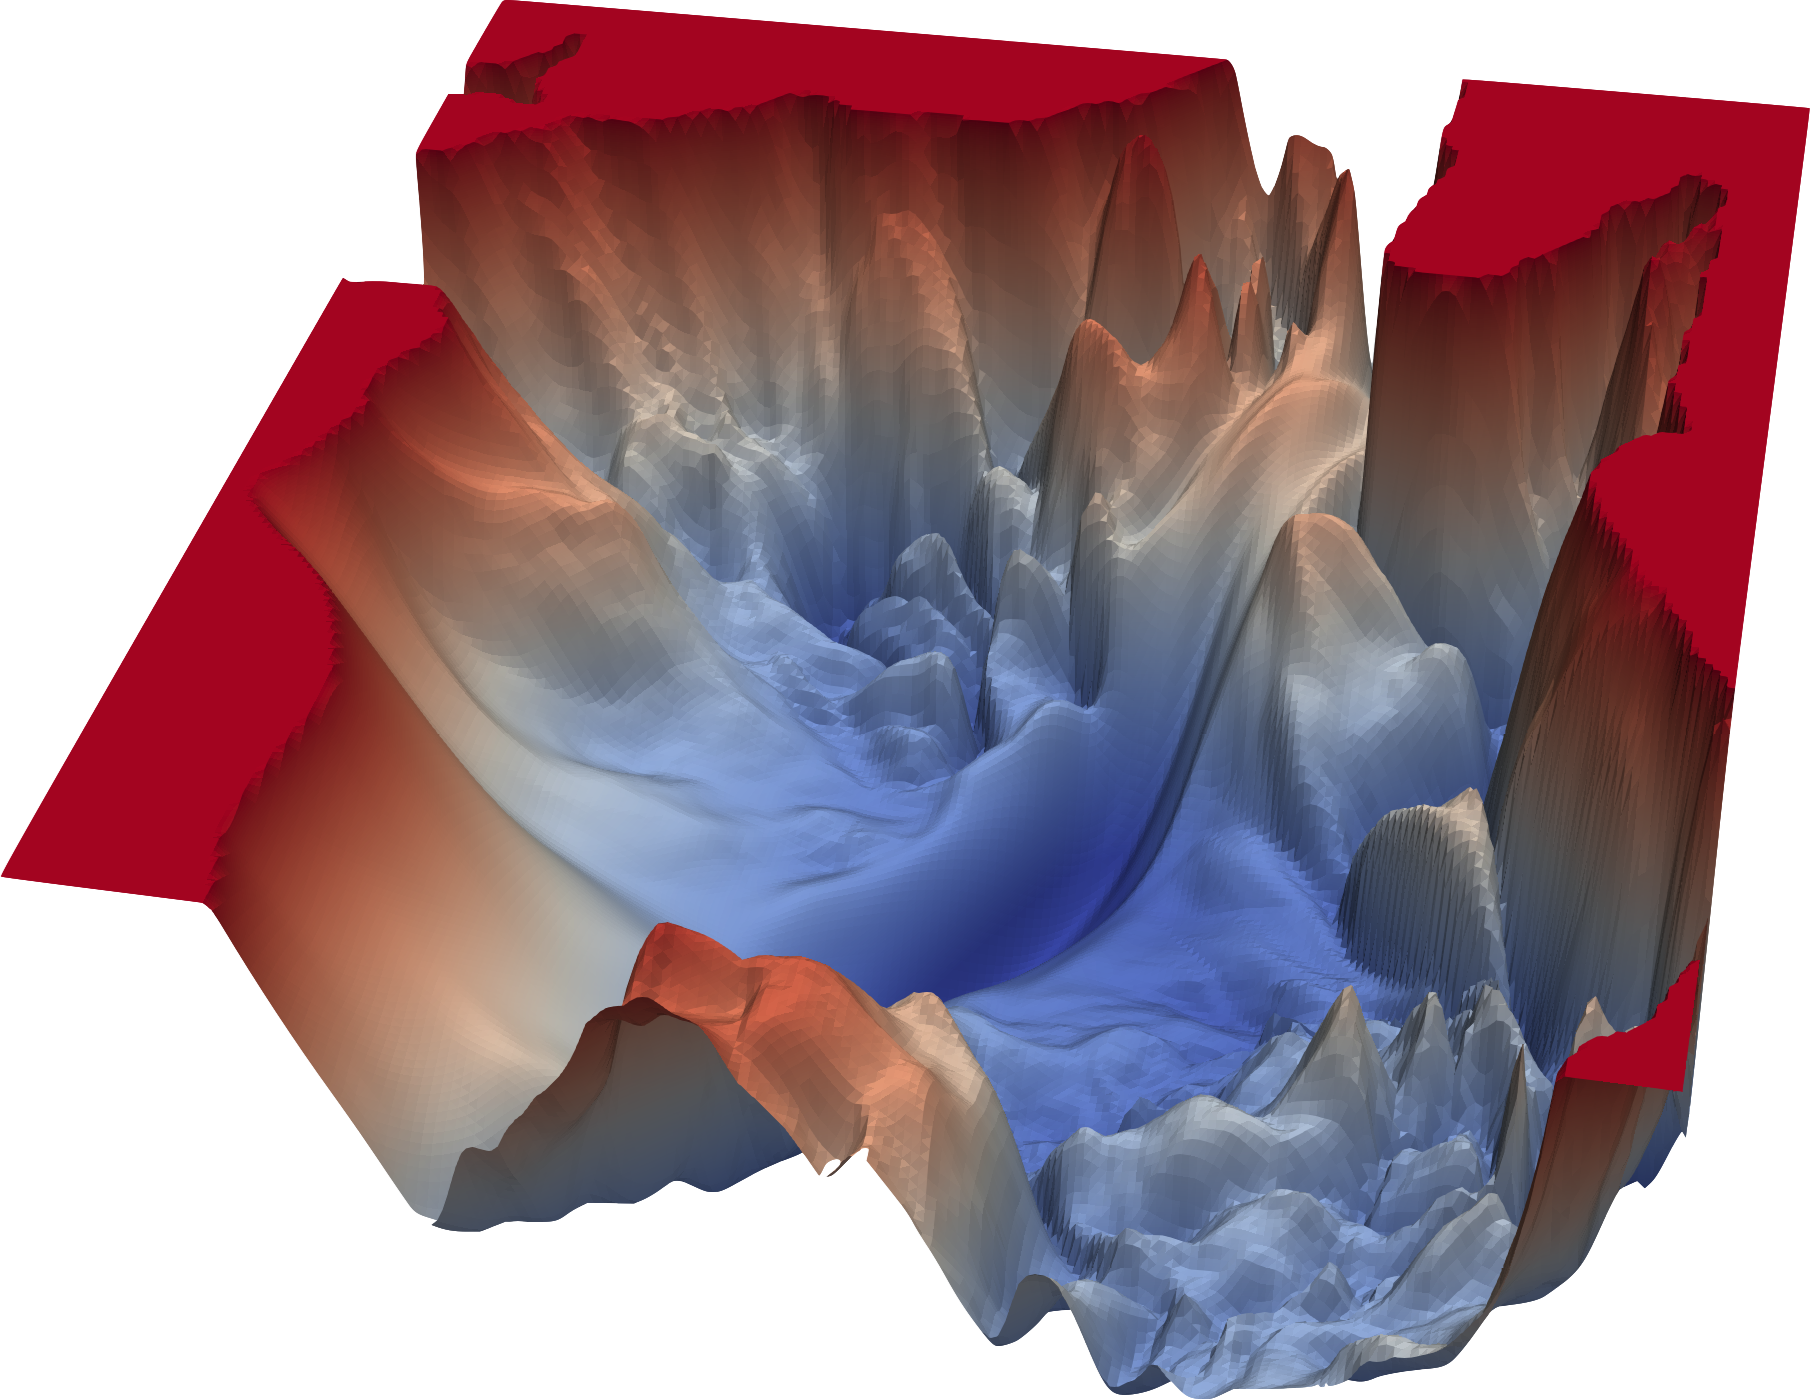
\includegraphics[width=.5\columnwidth]{../graphics/VGG56Loss}
\caption{Loss Function for VGG56 \cite{li2017visualizing}}
\end{figure}
\end{frame}


\begin{frame}{SGD with Learning Rate Schedule}
New problems.... new ideas!
\begin{itemize}
\item Fixing the Exponential Moving Decay \cite{dozat2016deep}
\item Cyclical Learning Rates \cite{smith2017cyclical}
\item Decay with restarts  \cite{loshchilov2016sgdr}
%\begin{figure}
%\includegraphics[width=.225\columnwidth]{../graphics/triangular}
%\includegraphics[width=.225\columnwidth]{../graphics/triangular2}\\
%\includegraphics[width=.225\columnwidth]{../graphics/LRRestarts}
%\includegraphics[width=.225\columnwidth]{../graphics/Snapshot}
%\caption{Schedules: Triangular  / Triangular with exponential decay / Exponential Decay with Restarts / Snapshot }
%\end{figure}
\item Snapshot Ensembles: Train 1, Get M for free \cite{huang2017snapshot}
%\item Learning with Random Learning Rates \cite{Blier2018}
\item Don't Decay the Learning Rate, Increase the batch size \cite{smith2018don}
\end{itemize}
\end{frame}





\begin{frame}{Optimizer in Keras}
\begin{figure}
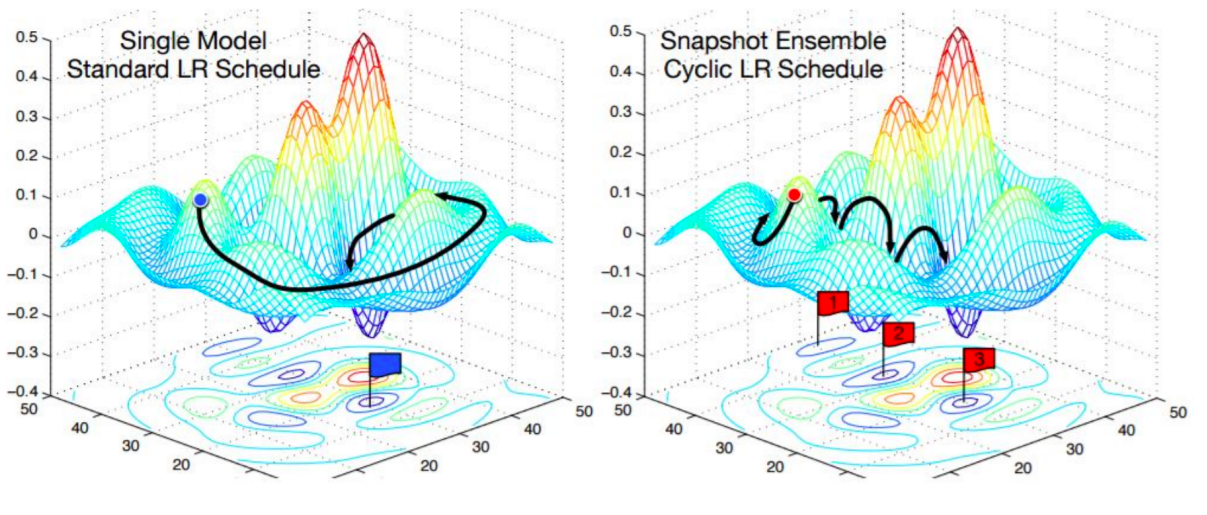
\includegraphics[width=.95\columnwidth]{../graphics/SnapshotCurve}
\caption{\cite{huang2017snapshot}}
\end{figure}
\begin{figure}
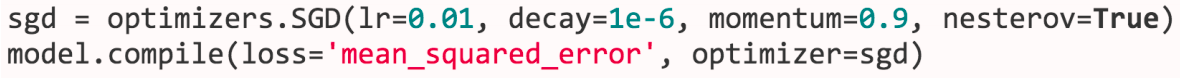
\includegraphics[width=.95\columnwidth]{../graphics/KerasSGD}
\end{figure}
%Practical Work 1:  Cyclic LR
\end{frame}


\begin{frame}{SGD with momentum \cite{Qian99}}
\begin{algorithm}[H]
\begin{algorithmic}[1]
\STATE \textbf{given} initial learning rate $\epsilon \in \mathbb{R}$, dataset $\X$, \alert{momentum factor $\beta_1 \in \mathbb{R}$}
\STATE \textbf{initialize} time step $t=0$, parameter vector $\param_{t=0} \in \mathbb{R}^\nfeatures$, first momentum factor $\mathbf{m}_{t=0}=0 \in \mathbb{R}^\nfeatures$, schedule multiplier $\eta_{t=0} \in \mathbb{R}$
\REPEAT
\STATE t=t+1
\STATE $\X_t=\texttt{SelectBatch} (\X)$ \begin{tiny}\texttt{Select a batch from data} \end{tiny}
\STATE $\mathbf{g}_t = \nabla f_t(\X_t,\param_{t-1})$ \begin{tiny}\texttt{Return parameter gradient} \end{tiny}
\STATE $\eta_t = $ SetScheduleMultiplier$(t)$ \begin{tiny}{Can be fixed,decay, warm restarts, ...}\end{tiny}
\STATE \alert{$\mathbf{m}_t = \beta_1 \mathbf{m}_{t-1} + \eta_{t} \eta  \mathbf{g}_t $}
\STATE $\param_i=\param_{t-1} - \alert{\mathbf{m}_{t}}$
\UNTIL stopping criterion is met
\RETURN optimized parameters $\param_i$
\end{algorithmic}
\caption{pseudocode for stochastic gradient descent \alert{with Momentum} }
\label{alg:seq}
\end{algorithm}
\end{frame}

\begin{frame}{Momentum}
\begin{figure}
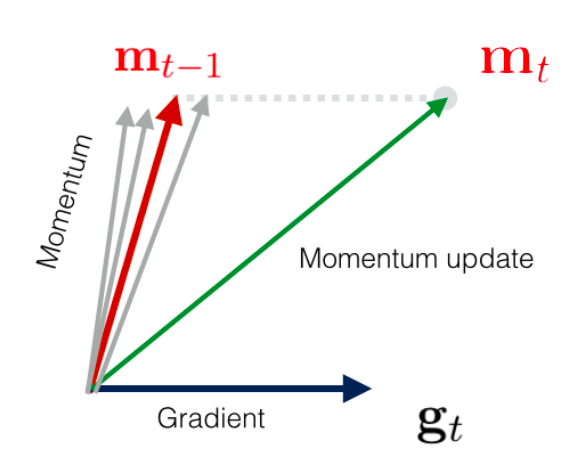
\includegraphics[width=.95\columnwidth]{../graphics/Momentum}
\end{figure}
\end{frame}

\begin{frame}{SGD with Nesterov's momentum \cite{Nesterov83}}
\begin{algorithm}[H]
\begin{algorithmic}[1]
\STATE \textbf{given} initial learning rate $\epsilon \in \mathbb{R}$, dataset $\X$, momentum factor $\beta_1 \in \mathbb{R}$
\STATE \textbf{initialize} time step $t=0$, parameter vector $\param_{t=0} \in \mathbb{R}^\nfeatures$, first momentum factor $\mathbf{m}_{t=0}=0 \in \mathbb{R}^\nfeatures$, schedule multiplier $\eta_{t=0} \in \mathbb{R}$
\REPEAT
\STATE t=t+1
\STATE $\X_t=\texttt{SelectBatch} (\X)$ \begin{tiny}\texttt{Select a batch from data} \end{tiny}
\STATE $\mathbf{g}_t = \nabla f_t(\X_t,\param_{t-1}\alert{+\mathbf{m}_{t-1}})$ \begin{tiny}\texttt{Return parameter gradient} \end{tiny}
\STATE $\eta_t = $ SetScheduleMultiplier$(t)$ \begin{tiny}{Can be fixed,decay, warm restarts, ...}\end{tiny}
\STATE $\mathbf{m}_t = \beta_1 \mathbf{m}_{t-1} + \eta_{t} \eta  \mathbf{g}_t $
\STATE $\param_i=\param_{t-1} - \mathbf{m}_{t}$
\UNTIL stopping criterion is met
\RETURN optimized parameters $\param_i$
\end{algorithmic}
\caption{pseudocode for stochastic gradient descent \alert{with Momentum} }
\label{alg:seq}
\end{algorithm}
\end{frame}

\begin{frame}{Nesterov's Momentum}
\begin{figure}
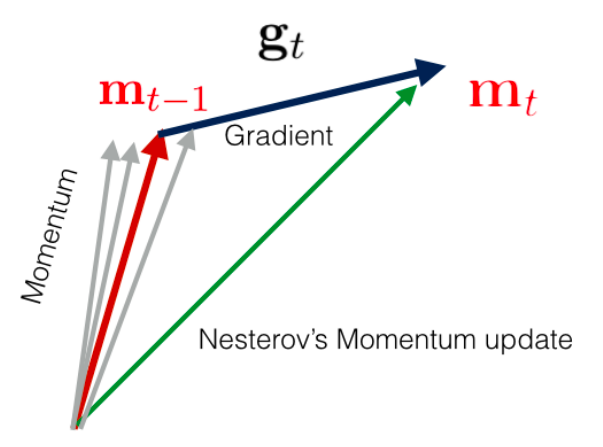
\includegraphics[width=.95\columnwidth]{../graphics/Nesterov}
\end{figure}
\end{frame}


\begin{frame}
\begin{table}[htp]
\caption{Summary: Some Optimizers I}
\begin{center}
\begin{tabular}{|c|c|} \hline
Method & Update\\ \hline
SGD  & $\param_{t+1}= \param_{t}-\eta\mathbf{g}(\param_{t})$ \\ \hline
Momentum    & $\param_{t+1}= \param_{t}+\mathbf{m}_t$, $\mathbf{m}_{t}= \alert{\beta_1 \mathbf{m}_{t-1}} -\eta \mathbf{g}(\param_{t}) $ \\  \hline
Nesterov Mom.  &  $\param_{t+1}= \param_{t}+\mathbf{m}_t$ , $\mathbf{m}_t= \beta_1 \mathbf{m}_{t-1} -\eta\mathbf{g}(\param_{t}+ \alert{\beta_1 \mathbf{m}_{t-1}}) $ \\ \hline
\end{tabular}
\end{center}
\label{default}
\end{table}%
%where $G_{ii,t}$ is the sum of the squares of the gradients of $\param_i$ up to time step $i$ while $\epsilon$ is a smoothing term that avoids division by zero.
%$\texttt{RMS}$ is the root mean squared error  (RMS)  of gradient for $\texttt{RMS}(g)_{t}$ or of parameter updates for $\texttt{RMS}(\partial \param)_{t}$ 
\end{frame}


\begin{frame}{Motivation}
\begin{enumerate}
\item SGD bounces around in high curvature directions and makes slow progress in low curvature directions. 
\begin{figure}
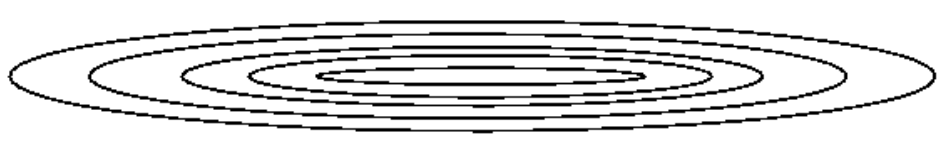
\includegraphics[width=.75\columnwidth]{../graphics/EllipsesValues}
\caption{Gradient Descent has poor performance on loss functions having contours that are very long "ellipsoids}
\end{figure}
\end{enumerate}
\end{frame}


\begin{frame}{Motivation: Invariance}
Suppose we would like to fit a linear regression on $y$ by using $\x=[x_1,x_2]$, i.e. $\hat{y}=w_1x_1+w_2x_2$:
\begin{table}[htdp]
\caption{default}
\begin{center}
\begin{tabular}{|c|c|c|}
$x_1$ & $x_2$ & $y$ \\
134.2 & 0.01234 & 1.2 \\
124.4 & 0.0294 & 2.2 \\
92.2& 0.0194 & 1.56 \\
$\vdots$ & $\vdots$ &$\vdots$ \\
98.2& 0.0214 & 1.76 \\
\end{tabular}
\end{center}
\label{default}
\end{table}%
\begin{enumerate}
\item This can happen since the inputs have arbitrary units.
\item Which weight, $w_1$ or $w_2$, should receive a larger gradient descent update?
\end{enumerate}
\end{frame}



\begin{frame}{Motivation}
\begin{enumerate}
\item SGD bounces around in high curvature directions and makes slow progress in low curvature directions. 
\item This can happen with highly correlated parameters.
\begin{figure}
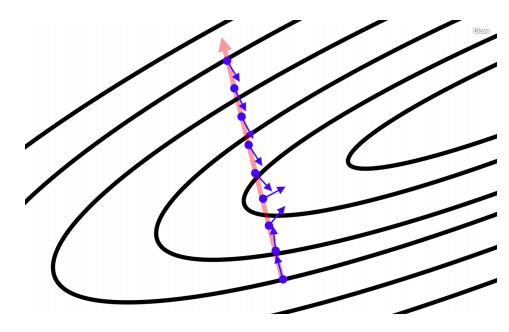
\includegraphics[width=.45\columnwidth]{../graphics/EllipseSGD}
%\includegraphics[width=.45\columnwidth]{../graphics/EllipseHSGD}
\caption{SGD}% \textbf{Right}: Natural Gradient Descent}
\end{figure}
\end{enumerate}
\end{frame}


\begin{frame}{Motivation}
\begin{figure}
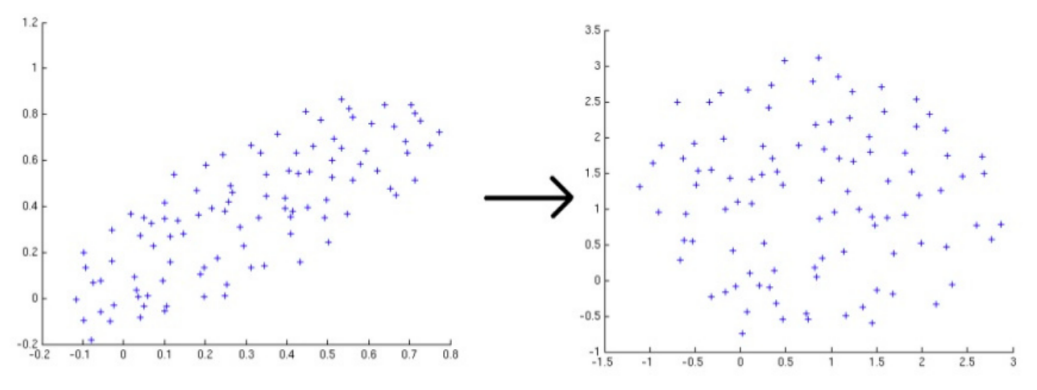
\includegraphics[width=.75\columnwidth]{../graphics/CorrelatedParameters}
%\includegraphics[width=.45\columnwidth]{../graphics/EllipseHSGD}
\caption{Which transformation can "decorrelate data? (Statistical Whitening Transform).}% \textbf{Right}: Natural Gradient Descent}
\end{figure}\pause
\alert{Inverse Covariance matrix do the work!}  \pause
Note that one can decompose $\boldsymbol{\Sigma}^{-1}$ into $\mathbf{V} \boldsymbol{\Lambda}^T \mathbf{V} ^{-1}$ (Singular value decomposition), then with $\boldsymbol{\Omega} = \{1 /\sqrt{\lambda_i} \}_{i=1}^{\nfeatures}$
\begin{eqnarray}
\x^T \boldsymbol{\Sigma}^{-1} \x =&\x^T \mathbf{V} \boldsymbol{\Omega\Omega}\mathbf{V}^{T}\x  \nonumber \\
=&(\boldsymbol{\Omega}\mathbf{V}^T\x)^T \boldsymbol{\Omega}\mathbf{V}^{T}\x \nonumber  \\ 
=&||\boldsymbol{\Omega}\mathbf{V}^T\x||_2^2 \label{EqNormInv}
\end{eqnarray} 
\alert{Euclidean distance in the projected space}
\end{frame}

\begin{frame}{From SGD to Natural Gradient Descend}
\begin{table}[htp]
\caption{Natural Gradient Descend  \cite{amari2000adaptive} }
\begin{center}
\begin{tabular}{|c|c|} \hline
Method & Update\\ \hline
SGD  & $\param_{t+1}= \param_{t}-\eta\mathbf{g}(\param_{t})$ \\ \hline
Natural Gradient Descend& $\param_{t+1}= \param_{t}-\eta \alert{\mathbf{\Sigma}_{\param_{t}}^{-1}} \mathbf{g}(\param_{t})$ \\ \hline
%Adagrad & $\param_{t+1}= \param_{t}- \frac{\eta}{\alert{\sqrt { G_{ii,t}+\epsilon  }}} \mathbf{g}(\param_{t})$  \\ \hline
\end{tabular}
\end{center}
\label{default}
\end{table}%
%where $G_{ii,t}$ is the sum of the squares of the gradients of $\param_i$ up to time step $i$ while $\epsilon$ is a smoothing term that avoids division by zero.
Two interpretations for the same method:
\begin{enumerate}
\item Second order optimization:  Newton Algorithm \cite{lecun2012efficient}
\item Gradient Descend in the Riemannian Manifold \cite{amari1998natural} = Fisher Information Matrix (empirical version)
\end{enumerate}
There are many other methods ... \alert{What is the problem with $\mathbf{\Sigma}_{\param}^{-1}$}?
\end{frame}

\begin{frame}{Adagrad}
In the Adagrad formulation \cite{duchi2011adaptive},
\begin{equation}
\param_{t+1}= \param_{t}- \frac{\eta}{\alert{\sqrt { G_{ii,t}+\epsilon  }}} \mathbf{g}(\param_{t})
\end{equation}
where $G_{ii,t}$ is the sum of the squares of the gradients of $\param_i$ up to time step $t$ while $\epsilon$ is a smoothing term that avoids division by zero.
$G_{ii,t}=\sum_{j=1}^{t}  \mathbf{g}^2_{i}(\param_{j})$, where $\mathbf{g}_{i}$ denote the i-th component of $\mathbf{g}$.\\
\alert{Note that only elements in the diagonal of $\mathbf{\Sigma}_{\param}^{-1}$ are estimated.}
\end{frame}

\begin{frame}{RMSprop \cite{hinton2012neural}}
In RMSprop \cite{hinton2012neural} proposes a rule update model's parameter by
\begin{equation}
\param_{t+1}= \param_{t}- \frac{\eta}{\alert{\sqrt { \texttt{RMS}(G_{ii})_{t}+\epsilon  }}} \mathbf{g}(\param_{t})
\end{equation}
where  $\texttt{RMS}(G_{ii,t})$ is a momentum estimation of $\sqrt { G_{ii,t}+\epsilon}$, i.e., 
defining the sequence 
\begin{equation*}
E(\mathbf{g}^2)_{t}=\rho E(\mathbf{g}^2)_{t-1} + (1-\rho) \mathbf{g}^2_t,
\end{equation*}
and we define $\texttt{RMS}(G_{ii,t})=E(\mathbf{g}^2)_{t}+\epsilon$.
\end{frame}

	
\begin{frame}{Adadelta \cite{zeiler2012adadelta}}
However, the unit in the learning rate don't correspondent with unit in the denominator. Thus, Adadelta optimiser \cite{zeiler2012adadelta} update by:
\begin{equation}
\param_{t+1}= \param_{t}- \frac{\alert{ \texttt{RMS}(\partial\param)_{t-1}}}{\alert{\sqrt { \texttt{RMS}(G_{ii,t}+\epsilon})}} \mathbf{g}(\param_{t})
\end{equation}
here is a diagonal matrix where each diagonal element $i,i$ is the sum of the squares of the gradients w.r.t. $\param_i$ up to time step  $t$
\end{frame}

\begin{frame}
\begin{table}[htp]
\caption{Summary: Some Optimizers II}
\begin{center}
\begin{tabular}{|c|c|} \hline
Method & Update\\ \hline
SGD  & $\param_{t+1}= \param_{t}-\eta\mathbf{g}(\param_{t})$ \\ \hline
Momentum    & $\param_{t+1}= \param_{t}+\mathbf{m}_t$, $\mathbf{m}_{t}= \alert{\beta_1 \mathbf{m}_{t-1}} -\eta \mathbf{g}(\param_{t}) $ \\  \hline
Nesterov Mom.  &  $\param_{t+1}= \param_{t}+\mathbf{m}_t$ , $\mathbf{m}_t= \beta_1 \mathbf{m}_{t-1} -\eta\mathbf{g}(\param_{t}+ \alert{\beta_1 \mathbf{m}_{t-1}}) $\\ \hline
Adagrad & $\param_{t+1}= \param_{t}- \frac{\eta}{\alert{\sqrt { G_{ii,t}+\epsilon  }}} \mathbf{g}(\param_{t})$  \\ \hline
RMSprop & $\param_{t+1}= \param_{t}- \frac{\eta}{\alert{\sqrt { \texttt{RMS}(G_{ii,t})+\epsilon  }}} \mathbf{g}(\param_{t})$  \\ \hline
Adadelta & $ \param_{t+1}= \param_{t}- \frac{\alert{ \texttt{RMS}(\partial\param)_{t-1}}}{\alert{\sqrt { \texttt{RMS}(G_{ii})_{t}+\epsilon  }}} \mathbf{g}(\param_{t})$ \\ \hline
\end{tabular}
\end{center}
\label{default}
\end{table}%
%where $G_{ii,t}$ is the sum of the squares of the gradients of $\param_i$ up to time step $i$ while $\epsilon$ is a smoothing term that avoids division by zero.
%$\texttt{RMS}$ is the root mean squared error  (RMS)  of gradient for $\texttt{RMS}(g)_{t}$ or of parameter updates for $\texttt{RMS}(\partial \param)_{t}$ 
\end{frame}


\begin{frame}{ADAM}
Adam can be looked at as a combination of RMSprop and Stochastic Gradient Descent with momentum \cite{kingma2014adam}
\begin{table}[htp]
\caption{Summary: Some Optimizers}
\begin{center}
\begin{tabular}{|c|c|} \hline
Method & Update\\ \hline
SGD  & $\param_{t+1}= \param_{t}-\eta\mathbf{g}(\param_{t})$ \\ \hline
Momentum    & $\param_{t+1}= \param_{t}+\mathbf{m}_t$, $\mathbf{m}_{t}= \alert{\beta_1 \mathbf{m}_{t-1}} -\eta \mathbf{g}(\param_{t}) $ \\  \hline
Nesterov Mom.  &  $\param_{t+1}= \param_{t}+\mathbf{m}_t$ , $\mathbf{m}_t= \beta_1 \mathbf{m}_{t-1} -\eta\mathbf{g}(\param_{t}+ \alert{\beta_1 \mathbf{m}_{t-1}}) $\\ \hline
Adagrad & $\param_{t+1}= \param_{t}- \frac{\eta}{\alert{\sqrt { G_{ii,t}+\epsilon  }}} \mathbf{g}(\param_{t})$  \\ \hline
RMSprop & $\param_{t+1}= \param_{t}- \frac{\eta}{\alert{\sqrt { \texttt{RMS}(G_{ii})_{t}+\epsilon  }}} \mathbf{g}(\param_{t})$  \\ \hline
Adadelta & $ \param_{t+1}= \param_{t}- \frac{\alert{ \texttt{RMS}(\partial\param)_{t-1}}}{\alert{\sqrt { \texttt{RMS}(G_{ii})_{t}+\epsilon  }}} \mathbf{g}(\param_{t})$ \\ \hline
ADAM&  Momentum  and RMSprop \\ \hline
NADAM&  Nesterov Momentum  and RMSprop \\ \hline
\end{tabular}
\end{center}
\label{default}
\end{table}%
\end{frame}

%\begin{frame}
%\cite{reddi2018convergence}
%\end{frame}

%\begin{frame}{Momentum}
%The momentum algorithm accumulates the exponentially decaying moving average of past gradients (called as velocity) and uses it as the direction in which to take the next step. Momentum is given by mass times velocity, which is equal to velocity if we’re using unit mass. The momentum update is given by:
%\end{frame}

%\begin{frame}{Nesterov Momemtum}
%Thus, it might be better to compute the gradient from that point onward
%\end{frame}



%%%%%%%%%%%%%%%%%%%%%%%%%%%%%%%%%%%%%%%%%%%%%%%%%%
\section{Difficulties in Deep Network Optimisation}

\begin{frame}{Difficulties in Deep Network Optimisation}
\begin{itemize}
\item[A]{Local minima / Global minima}
\item[B]{Saddle Point (Plateaus or Flat Regions)}
\item[C]{Vanishing Gradient}
\item[D]{Overfitting}
\item[E]{Initialization issues}
\end{itemize}
\end{frame}





\begin{frame}{Initialization Issues}
\begin{enumerate}
\item \textbf{Gaussian}: From Imagenet 2012, \cite{krizhevsky2012imagenet} recommends initialization with $\mathcal{N}(0,.01)$ and adding bias equal to one
for some layers become very popular. It is not possible to train very deep network from scratch with it \cite{simonyan2014very}. The problem is caused by the
activation (and/or) gradient magnitude in final layers \cite{he2016deep}.
\item  \textbf{Glorot}:  \cite{glorot2010understanding}  proposed a formula for estimating the standard deviation on the basis of
the number of input and output channels of the layers under assumption of no non-linearity between
layers. Despite invalidity of the assumption, Glorot initialization works well.	
\item \textbf{Orthogonal}: Saxe et al. \cite{saxe2013exact}  showed that orthonormal matrix initialization works much better
for linear networks than Gaussian noise, which is only approximate orthogonal. It also work fornetworks with non-linearities.
\item Recommended lecture: All you need is a good init  \cite{mishkin2015all}
\end{enumerate}
\end{frame}



\begin{frame}{Difficulties in Deep Network Optimisation}
\begin{itemize}
\item[C] {Vanishing Gradient:} If feedback signal has to be propagated through a deep stack of layers, the signal may become tenuous or even be lost entirely, rendering the network untrainable. During training, it causes the model's parameter to grow so large so that even a very tiny amount change in the input can cause a great update in later layers' output. The value of layer weights sometimes it overflow and the value becomes \alert{NaN}.
\end{itemize}
\end{frame}


\begin{frame}{Fighting against Vanishing Gradient \cite{pascanu2013difficulty}}
\begin{enumerate}
\item[1] Initialization of Weights: Don't initialize to values that are too large.
\item[2] Gradient clipping: clips parameters gradients during backpropation by a maximum value or maximum norm 
\begin{figure}
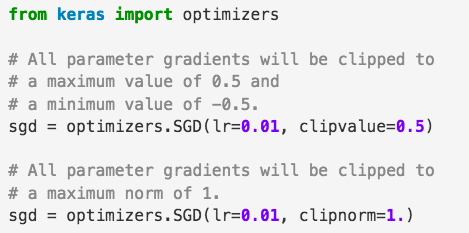
\includegraphics[width=.75\columnwidth]{../graphics/KerasClip}
\end{figure}
\end{enumerate}
\end{frame}

\begin{frame}{Fighting against Vanishing Gradient}
\begin{enumerate}
\item[3] Skip connections or Shortcuts (Residual Networks): 
\begin{figure}
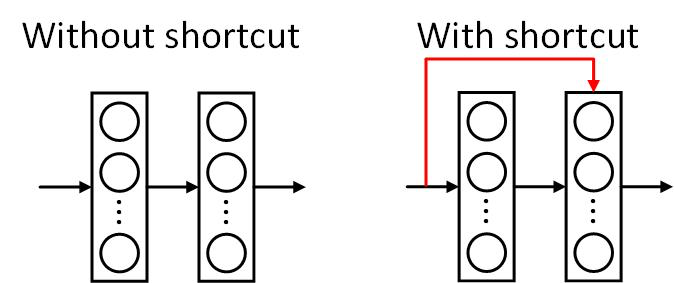
\includegraphics[width=.65 \columnwidth]{../graphics/shortcut}
\end{figure}
\end{enumerate}
\begin{figure}
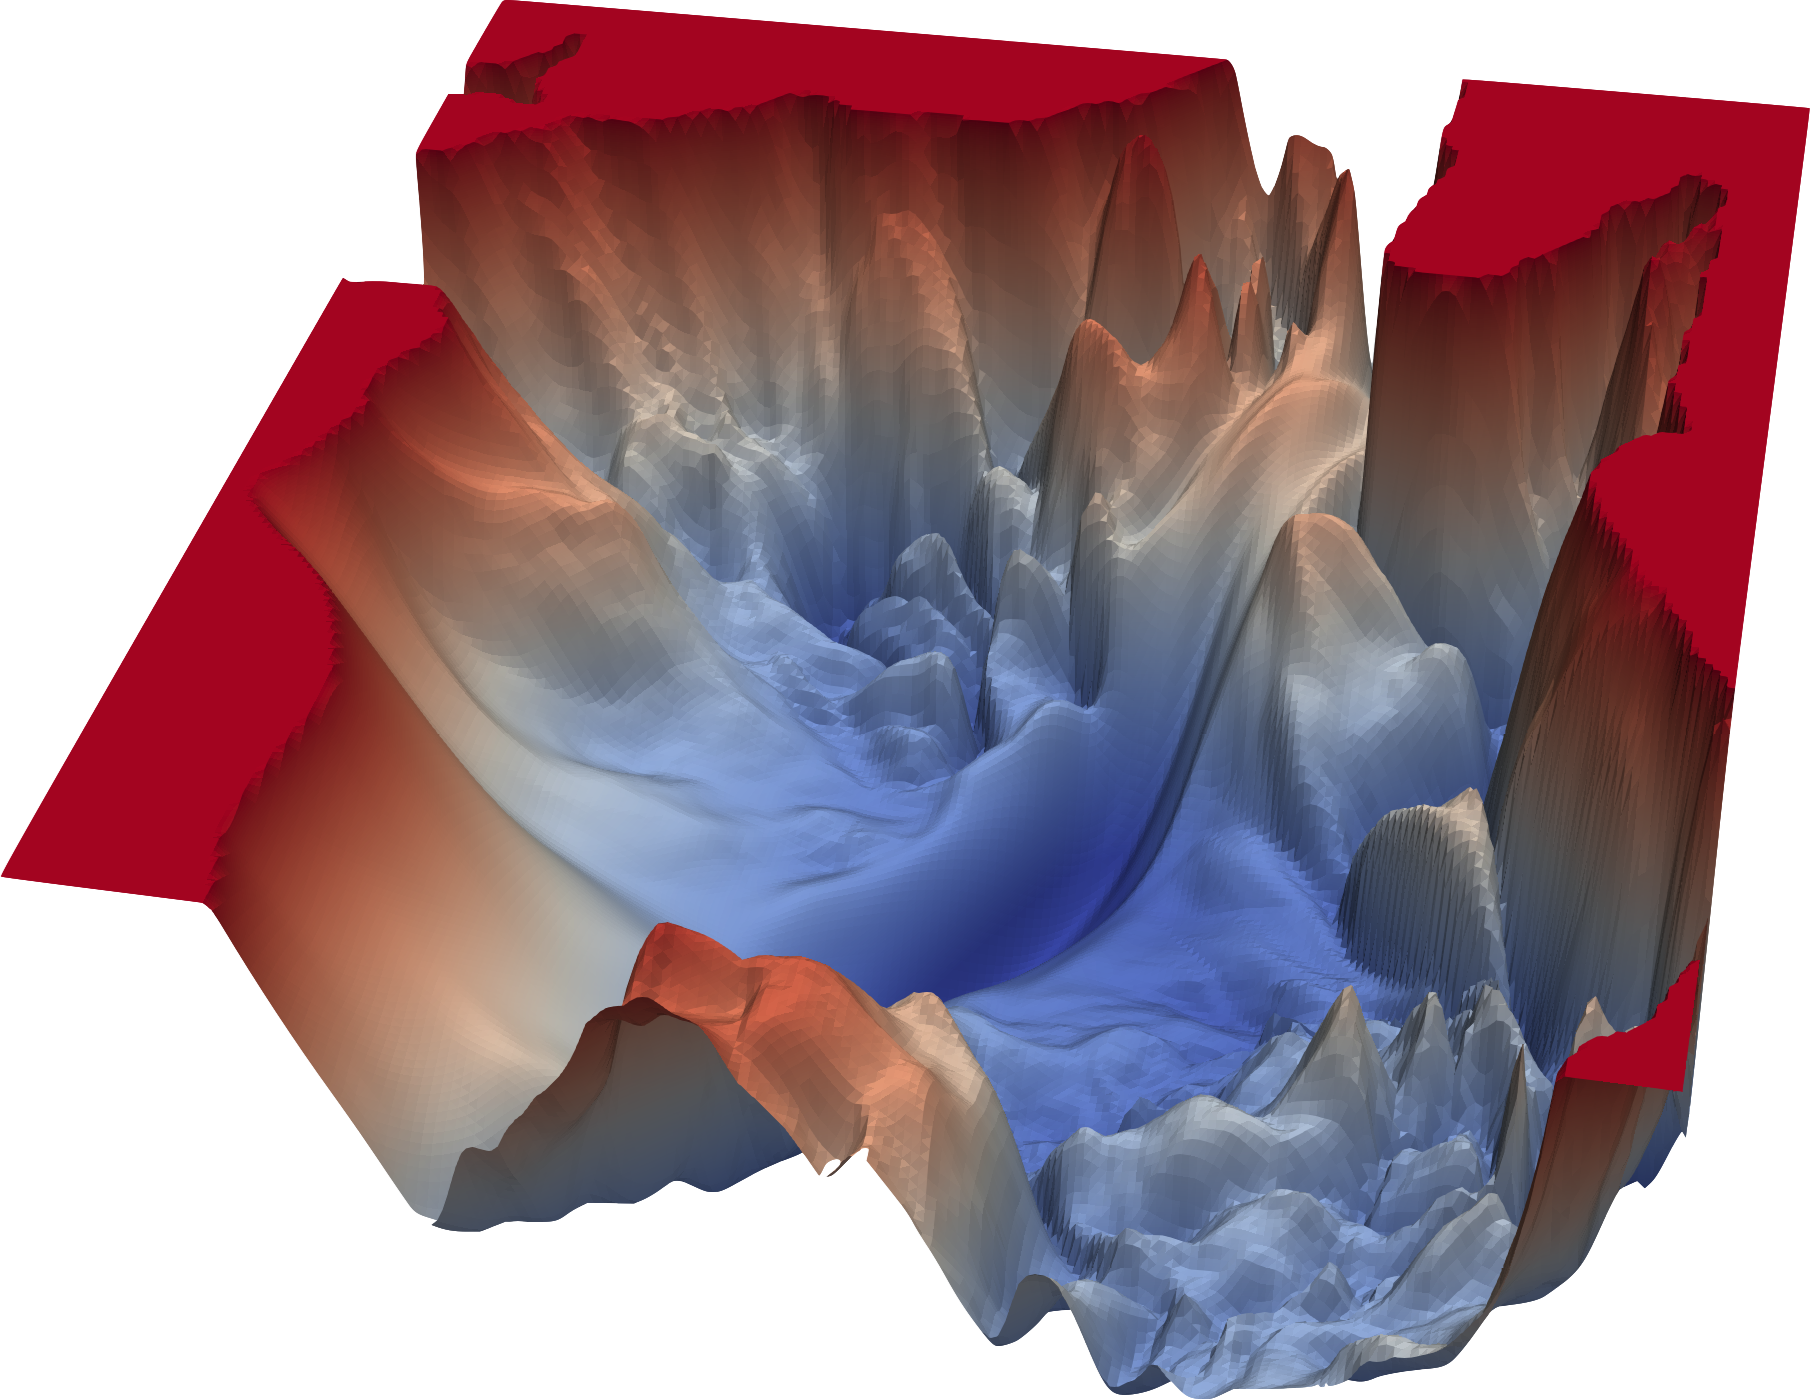
\includegraphics[width=.4\columnwidth]{../graphics/VGG56Loss}
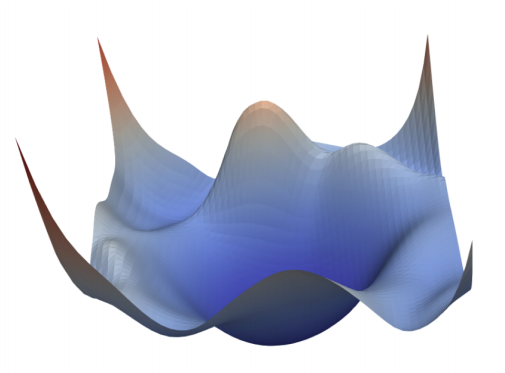
\includegraphics[width=.45\columnwidth]{../graphics/Resnet56}
\caption{From \cite{li2017visualizing}}
\end{figure}


\textbf{Visualizing the Loss Landscape of Neural Net}, \cite{li2017visualizing}

\end{frame}

\begin{frame}{Fighting against Vanishing Gradient}
\begin{enumerate}
\item[4] Avoid "stuck states" induced by activation function: 
\begin{figure}
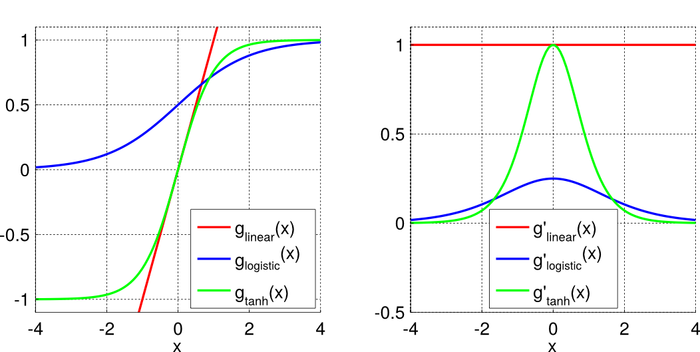
\includegraphics[width=.85 \columnwidth]{../graphics/nnet-error-functions2}
\caption{Left: Three activation function Right: Derivative of activation function.}
\end{figure}
\end{enumerate}
\end{frame}

\begin{frame}{Fighting against Vanishing Gradient}
\begin{enumerate}
\item[5] Regularization: $L_2$ or $L_1$ norm applies "weight decay" in the cost function of the network. Note that for many activation function, when the activation value is small, that will be almost linear.
\begin{figure}
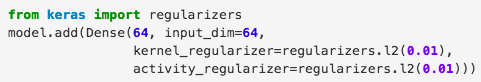
\includegraphics[width=.75 \columnwidth]{../graphics/KerasRegularizer}
\end{figure}

\end{enumerate}
\end{frame}


\begin{frame}{Batch Normalization \cite{ioffe2015batch}  \cite{mishkin2015all}}
BatchNorm (BN) is a transformation applied before the applying activation in a given layer, i.e. if $x_i$ are the output of a layer for a mini-batch, the BN is defined by
\begin{eqnarray*}
\hat{x}_i = \frac{x_i-\mu_{B}}{\sqrt{\sigma^2_B}}, \quad \quad
BN_{\gamma,\beta}(x_i):= \gamma \hat{x}_i + \beta
\end{eqnarray*}
where $\mu_{B}$ and $\sigma^2_B$ are respectively the mini-batch mean and variance. $\gamma$ scale and $\beta$ shift a learned parameters.
\begin{itemize}
\item Moving values to zero (activation works better!) 
\item Large learning rates can scale the parameters which could amplify the gradients, thus leading to an explosion. In Batch normalization small changes in parameter to one layer do not get propagated to other layers. 
\item This makes it possible to use higher learning rates for the optimizers, which otherwise would not have been possible. 
\item It also makes gradient propagation in the network more stable.
\end{itemize}
\end{frame}


\begin{frame}{Batch Normalization}
\begin{figure}
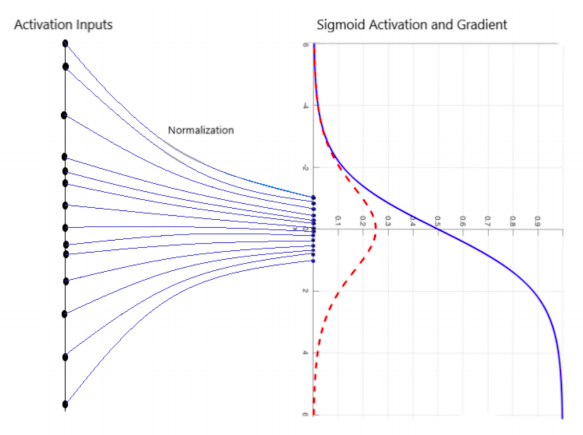
\includegraphics[width=.75 \columnwidth]{../graphics/BatchNormalization}
\caption{Image from "Intuit and Implement: Batch Normalization"}
\end{figure}
\end{frame}
%\begin{itemize}
%\item[D]{Ill-conditioning of the Hessian Matrix}
%\end{itemize}
%\end{frame}

%%%%%%%%%%%%%%%%%%%%%%%%%%%%%%%%%%%%%%%%%%%%%%%%%%


\section{How to fight against overfitting}


\begin{frame}{Supervised Learning (Machine Learning)}
\begin{itemize}
\item \textbf{Data}: $\nsize$ observations $(\x_i,y_i) \in \mathcal{X} \times \mathcal{Y}, i=1,\ldots,\nsize$, \alert{\textbf{i.i.d.}}
\item \textbf{Model}: $\texttt{Model}(\x):=\param^T\featmap (\x)$ of features  $\featmap (\x) \in \mathbb{R}^\nfeatures$ \alert{Prediction as linear mapping of features}
\item \textbf{Minimization of Regularized Empirical Risk}: We would like to find $\param^{*}$ the solution of:
\begin{eqnarray*}
\param^{*}:=\min_{\param \in \mathbb{R}^\nfeatures} \frac{1}{\nsize} \sum_{i=1}^{\nsize} \loss(y_i,\param^T\featmap (\x_i))&  + &\alpha \mathcal{R}(\param) \\
\texttt{Data fitting}& + &\texttt{regularizer}
\end{eqnarray*}
\end{itemize}
where $\loss(\cdot,\cdot)$ is called the  \emph{loss function}.
\end{frame}



\begin{frame}{Other loss functions, other models}
%\begin{center}\includegraphics[width=.2\columnwidth]{../graphics/Loss}\end{center}
\begin{enumerate}
\item Support Vector Machine (SVM): "Hinge" Loss 
\begin{equation}
\loss(y,\param^T\featmap(\x))=\max \{1-y\param^T\featmap(\x),0\}
\end{equation}
\item Logistic Regression: 
\begin{equation}
\loss(y,\param^T\featmap(\x))=\log (1+\exp (-y\param^T\featmap(\x)))
\end{equation}
\item Mean Squared Regression:
\begin{equation}
\loss(y,\param^T\featmap(\x))=\frac{1}{2}(y-\param^T\featmap(\x))^2
\end{equation}
\item Adaboost
\begin{equation}
\loss(y,\param^T\featmap(\x))=\exp^{ -(y-\param^T\featmap(\x))}
\end{equation}
\item Others ...
\end{enumerate}
\end{frame}

\begin{frame}{Minimizing Empirial Risk = Problems!}
\begin{itemize}
\item Empirical Risk: $\hat{f}(\param) :=\frac{1}{\nsize} \sum_{i=1}^{\nsize} \loss(y_i,\param^T\featmap (\x_i))$ \pause \\\alert{Loss in a training set}
\end{itemize}
\begin{figure}[htb]
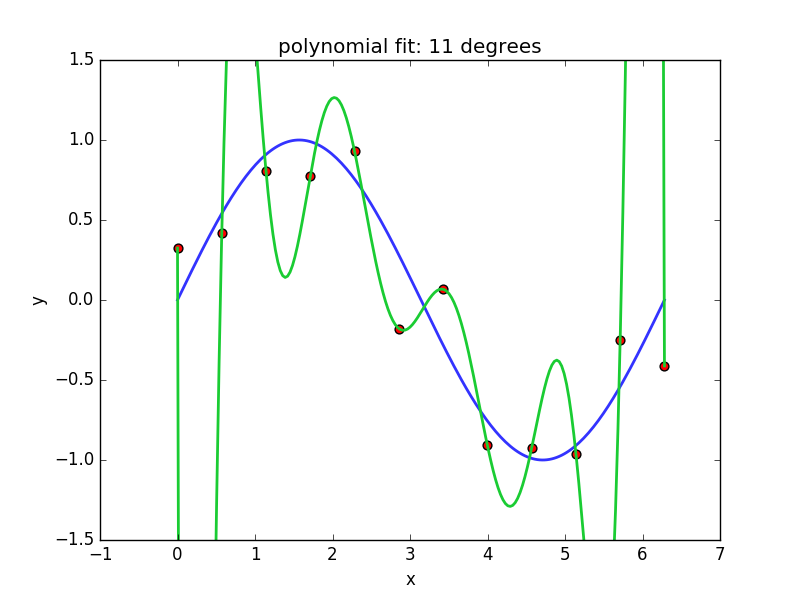
\includegraphics[width=0.4\textwidth]{../graphics/polyfit_degree_11.png}
\caption{There are infinity minimizer of the empirical risk!}
\end{figure}
 \pause
\begin{itemize}
\item Expected Risk : $f(\param) := \mathbb{E}_{(\x,y)} \loss(y,\param^T\featmap (\x))$ \pause  \\\alert{Loss in a testing set}
\end{itemize}
There are infinity minimizers of the empirical risk, but most of them have a large expected risk (\alert{overfitting}).
\end{frame}


\begin{frame}{Bias/Variance Tradeoff}
Let $\hat{y}:=\texttt{Model}(\x)$ the prediction of a deterministic model evaluated at $\x$
\begin{eqnarray*}
\mathbb{E}_{(\x,y)}\left [ (y-\texttt{Model}(\x))^ 2\right ] = \\ Var\left[y \right] + Var \left[ \texttt{Model}(\x) \right] + (Bias [\texttt{Model}(\x)])^2
\end{eqnarray*}
\begin{figure}
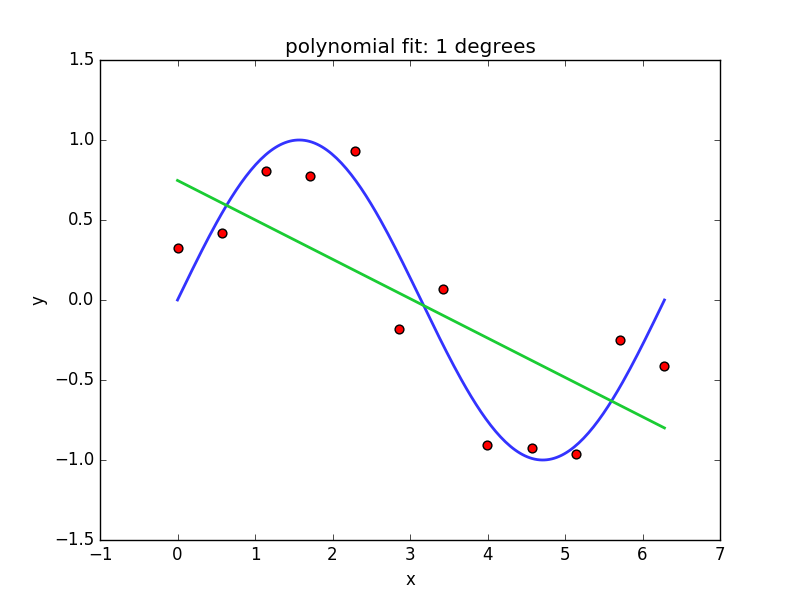
\includegraphics[width=.45 \columnwidth]{../graphics/polyfit_degree_1}
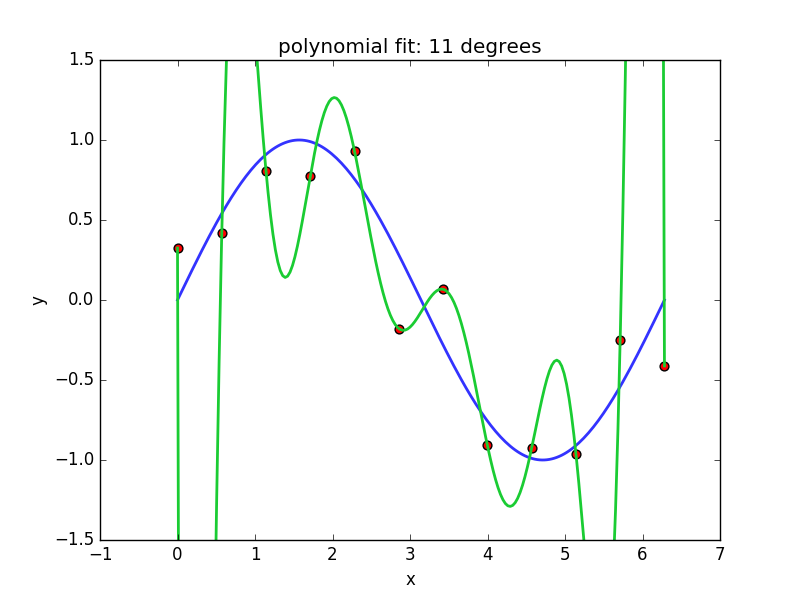
\includegraphics[width=.45 \columnwidth]{../graphics/polyfit_degree_11}
\caption{Underfitting / Overfitting}
\end{figure}
Underfitting : Prediction with less variance but more bias
Overfitting : Prediction with more variance but less bias
\end{frame}

\begin{frame}{How to judge if a deep machine learning model is overfitting or not?}
\begin{columns}
\begin{column}{.5\textwidth}
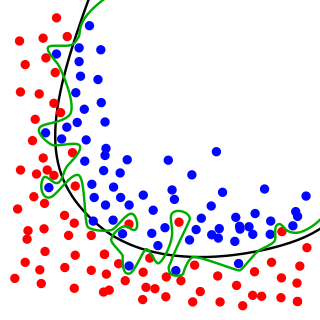
\includegraphics[width=.95 \columnwidth]{../graphics/Overfitting}
\end{column}
\begin{column}{.5\textwidth}
\begin{itemize}
\item Training Set / Testing Set
\item Cross-Validation
\item $||\param||_p$ is large
\end{itemize}
\end{column}
\end{columns}
\end{frame}

\begin{frame}{1. Early Stopping / ReduceLROnPlateau / Learning Rate Scheduler}
\begin{figure}
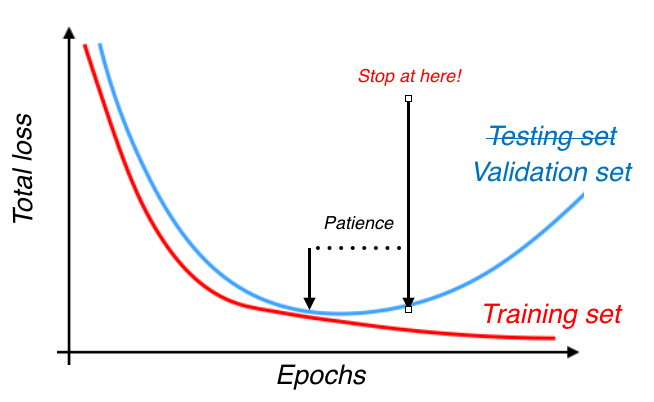
\includegraphics[width=.75 \columnwidth]{../graphics/EarlyStopping}
\end{figure}
\end{frame}

\begin{frame}{1. Early Stopping / ReduceLROnPlateau / Learning Rate Scheduler}
\begin{figure}
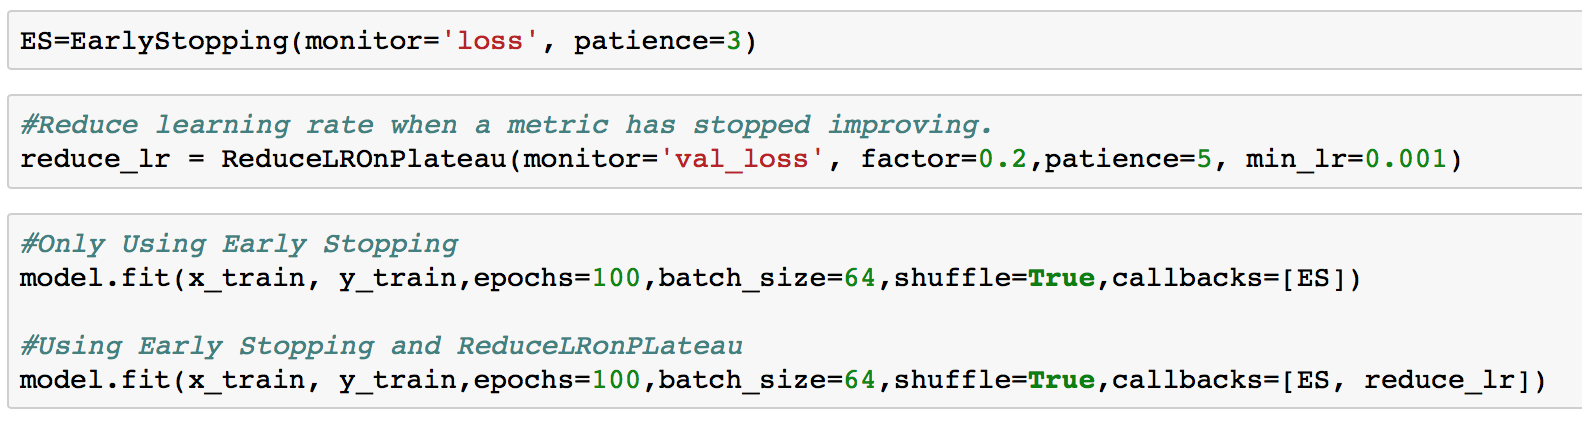
\includegraphics[width=1 \columnwidth]{../graphics/CallBacksKeras}
\caption{Callbacks in Keras}
\end{figure}
\end{frame}

\begin{frame}{2. We need more data!}
\begin{figure}
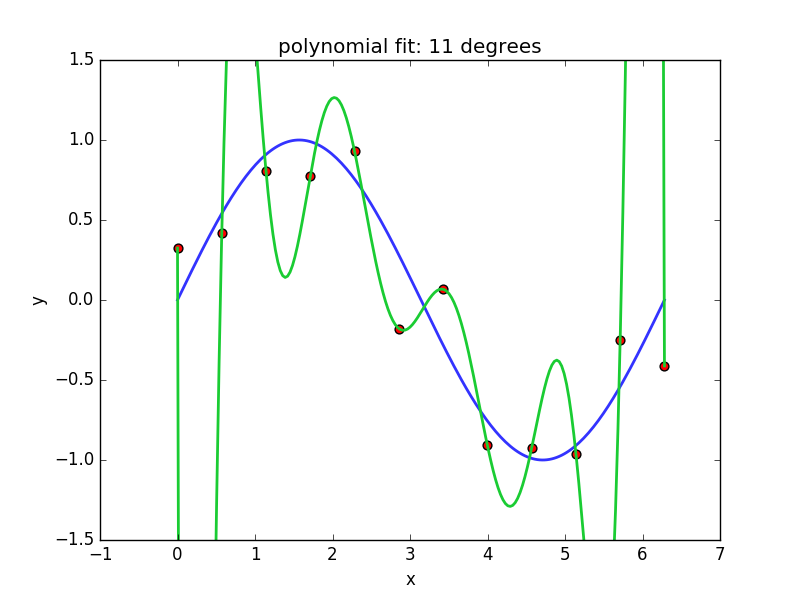
\includegraphics[width=.45 \columnwidth]{../graphics/polyfit_degree_11}
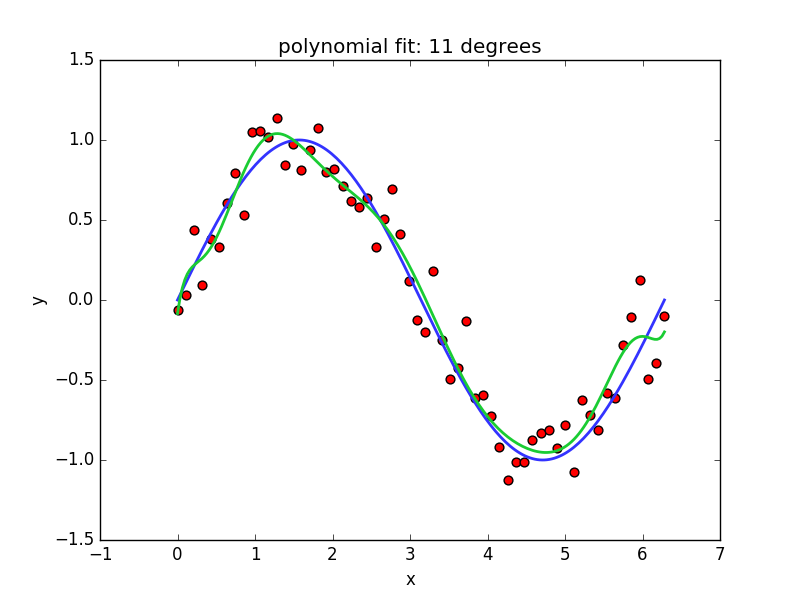
\includegraphics[width=.45 \columnwidth]{../graphics/polyfit_degree_11_N60.png}
\caption{Same model complexity but more data}
\end{figure}
\begin{enumerate}
\item Additive Gaussian noise.
\item Data augmentation.
\item Adversarial Training (Not in this talk)
\end{enumerate}
\end{frame}

\begin{frame}{Expected Risk (again)}
The expected risk
\begin{equation*}
 \mathbb{E}_{(\x,y)}  \loss(y,\texttt{Model}) =  \int \loss(y,\texttt{Model} (\x)) dP(\x,y) := R(\texttt{Model} )
\end{equation*}
\pause
But the distribution P is \alert{unknown} in most practical situations. 
\pause
We usually have access to a set of training data $T=\{(\x_i,y_i) \}_{i=1}^{\nsize}$, where $(\x_i,y_i)\sim P$, for all $i=1,\ldots,\nsize$. Thus, we may approximate $P$ by the \emph{empirical distribution}:
\begin{equation*}
P_{\delta}(\x,y) = \frac{1}{\nsize}\sum_{i=1}^{\nsize}\delta(\x=\x_i,y=y_i)
\end{equation*}
\end{frame}

\begin{frame}{Empirical Risk (again)}
Using the empirical distribution $P_{\delta}$, we can now approximated the expected risk, by the called \emph{empirical risk}
\begin{equation}\label{RM}
R_{\delta}(\texttt{Model} ) = \int \loss(y,\texttt{Model} (\x)) dP_{\alert{\delta}}(\x,y) = \frac{1}{\nsize}\sum_{i=1}^{\nsize}\loss(\texttt{Model}(\x_i),y_i)
\end{equation} \\
Learning the function $f$ by minimizing \eqref{RM} is known as the Empirical Risk Minimization (ERM) principle \cite{vapnik98} (Vapnik, 1998). If the number of parameters are comparable to $\nsize$, one trivial way to minimize \eqref{RM} is to \alert{memorize} the whole set of training data (overfitting).
\end{frame}

\begin{frame}{Vicinal Risk Minimization (VRM)}
$P_{\delta}$ is only one of the possibility to approximate the true distribution $P$. \cite{chapelle2001vicinal} proposed to approximate $P$ by:
\begin{equation*}
P_{v}(\x,y) = \frac{1}{\nsize}\sum_{i=1}^{\nsize}v(\tilde{\x},\tilde{y}, |\x_i,y_i)
\end{equation*}
where $v$ is \emph{vicinity distribution} that measure the probability for a "virtual" pair $(\tilde{\x},\tilde{y})$ to be in the \emph{vicinity} of the training pair $(\x,y)$. \pause
\begin{enumerate}
\item[1]  Gaussian vicinities: $v(\tilde{\x},\tilde{y}, |\x_i,y_i)=\mathcal{N}(\tilde{\x}-\x,\sigma^2\mathbf{I})\delta(\tilde{y}=y)$
\end{enumerate}
\pause
\alert{which is equivalent to augmenting the training data with additive Gaussian noise}
\end{frame}

\begin{frame}{Keras Gaussian Layer}
\begin{figure}
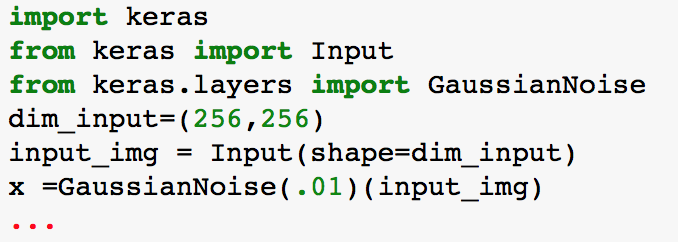
\includegraphics[width=.95 \columnwidth]{../graphics/GaussianNoiseLayer}
\caption{Gaussian vicinities in Keras}
\end{figure}
\end{frame}

\begin{frame}{Why Data-augmentation?}
\begin{enumerate}
\item[2]  Data-augmentation based vicinities: $P_{agg}(\x,y) = \frac{1}{\nsize}\sum_{i=1}^{\nsize}\delta(\tilde{\x},y_i)$, where $\tilde{\x}$ is a random transformation applied $\x$
\end{enumerate}
\begin{figure}
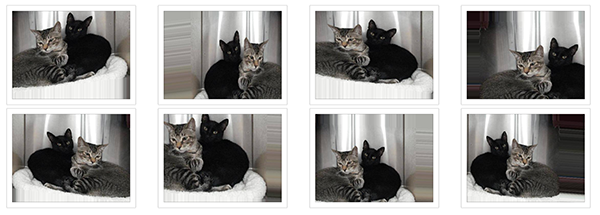
\includegraphics[width=.99 \columnwidth]{../graphics/cat_data_augmentation}
\caption{Example of a set of image produce by random transformations (translations, rotations, zooming, ...)}
\end{figure}
\end{frame}

\begin{frame}
\begin{figure}
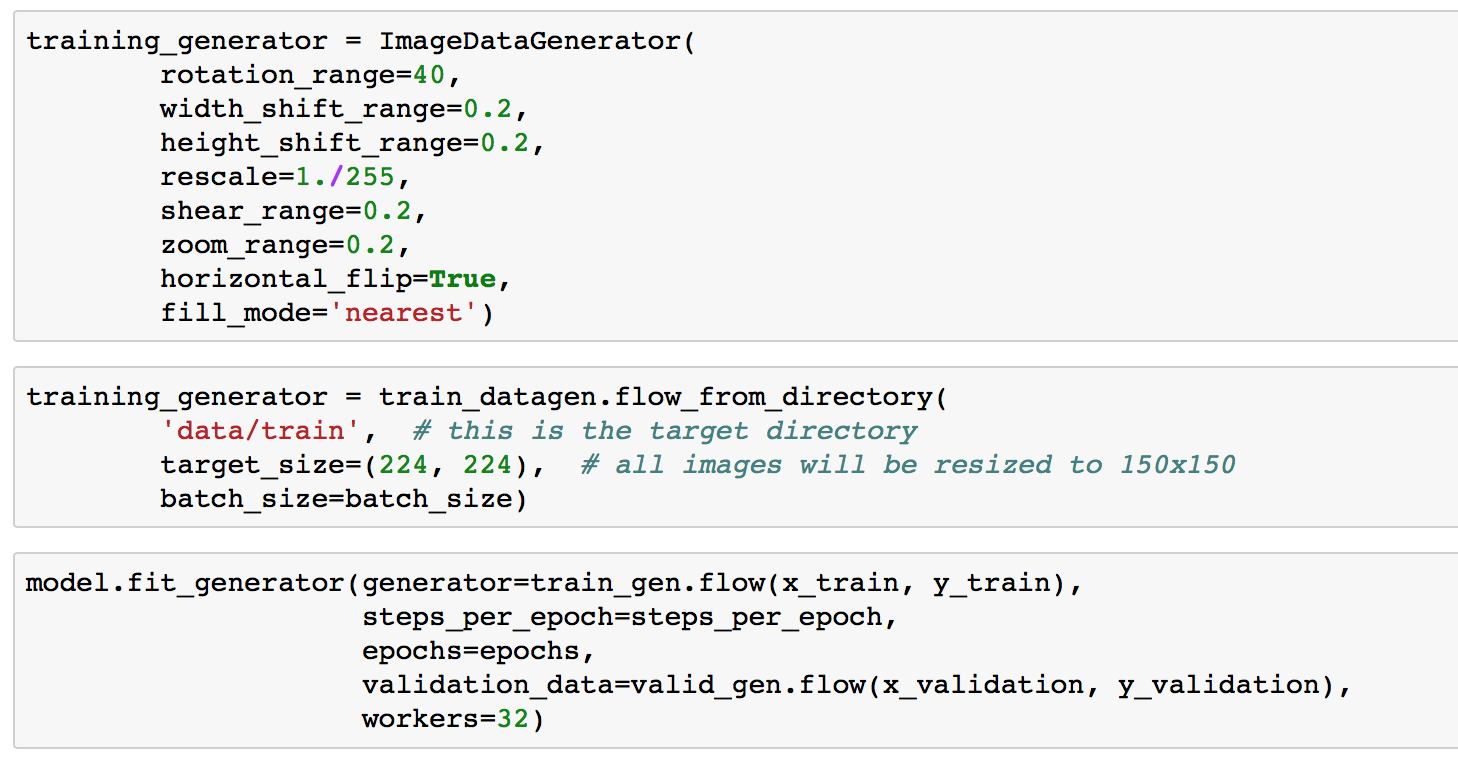
\includegraphics[width=.99 \columnwidth]{../graphics/DataGeneratorKeras}
\caption{Data Generator in Keras}
\end{figure}
\end{frame}

\begin{frame}{Regularization vs Overfitting}
\begin{enumerate}
\item "Weight Decay": Again?
\item Early Stopping
\item More data! : Data Augmentation
\item More data!  : Adversarial Examples
\item Summing-up: Dropout
\end{enumerate}
\end{frame}

\begin{frame}{How can we reduce the variance of ?}
\begin{itemize}
\item Remember: given $\nsize$ i.i.d. obsevations $\x_1,\x_2,\ldots,\x_\nsize$ each of them with variance equal to $\sigma^2$. 
\item What is the variance of $\bar{\x}=\frac{1}{\nsize} \sum_{i=1}^{\nsize} \x_i $? \pause $\frac{\sigma^2}{\nsize}$
\item \alert{Hint}: Train model on different training sets, and use the mean of predictions as final model of prediction.
\end{itemize}
\end{frame}

\begin{frame}{Dropout: \cite{srivastava2014dropout} }
\begin{figure}
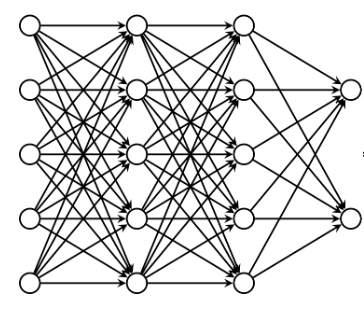
\includegraphics[width=.45 \columnwidth]{../graphics/NetworkDropoutNO}
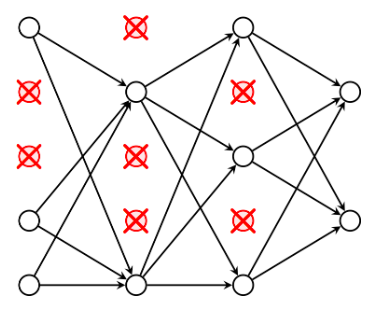
\includegraphics[width=.45 \columnwidth]{../graphics/NetworkDropoutYes}
\caption{Left: No Dropout Right: Dropout}
\end{figure}
\begin{itemize}
%\item Since dropout can be seen as a stochastic regularization technique
\item Avoid memorization!
\item Dropout forces to learn more robust features that are useful in conjunction with many different random subsets.
\item With $H$ hidden units, each of which can be dropped, we have $2^H$ possible models!
\end{itemize}
%Dropout: a simple way to prevent neural networks from overfitting. 2014
\end{frame}

\begin{frame}{Dropout}
\begin{figure}
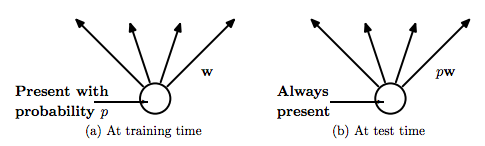
\includegraphics[width=.85 \columnwidth]{../graphics/DropoutP}
\caption{Left: A unit at training time that is present with probability $p$ and is connected to units
in the next layer with weights $\mathbf{W}$. Right: At test time, the unit is always present and
the weights are multiplied by $p$. The output at test time is same as the expected output
at training time.}
\end{figure}
\end{frame}


\begin{frame}{Dropout}
\begin{figure}
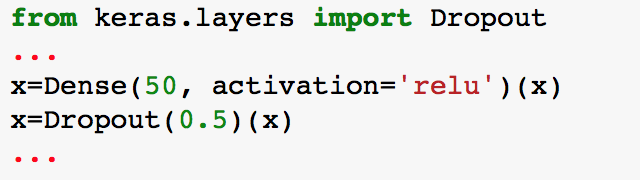
\includegraphics[width=.99 \columnwidth]{../graphics/DropoutKeras}
\caption{Dropout in Keras. Layer with a dropout of $p=.5$}
\end{figure}
Practical Work 2:  Dropout on Fashion MNIST
\end{frame}
	

%%%%%%%%%%%%%%%%%%%%%%%%%%%%%%%%%%%%%%%%%%%%%%%%%%
%%%%%%%%%%%%%%%%%%%%%%%%%%%%%%%%%%%%%%%%%%%%%%%%%%
%%%%%%%%%%%%%%%%%%%%%%%%%%%%%%%%%%%%%%%%%%%%%%%%%%

\section{References}
\begin{frame}[allowframebreaks]
	\frametitle{References}
	\bibliography{slides_deep.bib}
\end{frame}

\end{document}
